\section{Reynolds Stress Analysis}
\label{ch:reynolds}

Open from `3.\ Analysis $\to$ Reynolds Stresses`.

In turbulent flows, the instantaneous velocity can be decomposed into a time-averaged mean $\langle U_i \rangle$ and a fluctuating component $u'_i$, such that $U_i = \langle U_i \rangle + u'_i$. The Reynolds stress tensor $\langle u'_i u'_j \rangle$ quantifies the statistical intensity and directionality of these fluctuations and appears as a closure term in the Reynolds-Averaged Navier-Stokes (RANS) equations (Pope, 2000):
\[
\rho \frac{D \langle U_i \rangle}{Dt} = -\frac{\partial \langle p \rangle}{\partial x_i} + \mu \nabla^2 \langle U_i \rangle - \rho \frac{\partial \langle u'_i u'_j \rangle}{\partial x_j}
\]
The diagonal components $\langle u'u' \rangle$, $\langle v'v' \rangle$, $\langle w'w' \rangle$ are the normal stresses, directly related to the turbulent kinetic energy by $k = \tfrac{1}{2}(\langle u'u'\rangle + \langle v'v'\rangle + \langle w'w'\rangle)$. The off-diagonal components $\langle u'v' \rangle$, $\langle u'w' \rangle$, $\langle v'w' \rangle$ are the shear stresses, which are responsible for the turbulent momentum transfer across shear layers and boundary layers.

For 2D2C data, only $\langle u'u' \rangle$, $\langle v'v' \rangle$, and $\langle u'v' \rangle$ are available. All six components are computed for stereo (2D3C) data.

\begin{quote}
\textbf{Tip}
The shear stress $\langle u'v' \rangle$ is particularly useful for identifying shear layers and recirculation zones: it changes sign across the centreline of a jet or shear layer, and its peak magnitude locates the region of maximum turbulent momentum transfer.
\end{quote}

\noindent\textbf{Reference:} Pope, S.B. (2000). \textit{Turbulent Flows}. Cambridge University Press.

\subsection{2D contour map}

\begin{quote}
\textbf{Important}
\begin{enumerate}[leftmargin=1.5em, topsep=2pt]
  \item Select `2D Contour Map` under Plot Mode.
  \item Choose the component from the `Component` dropdown.
  \item Optionally check `Scale by $U_m^2$` and enter the bulk velocity $U_m$ to non-dimensionalise.
  \item Click `Plot Contour`.
\end{enumerate}
\end{quote}

\begin{figure}[htbp]
  \centering
  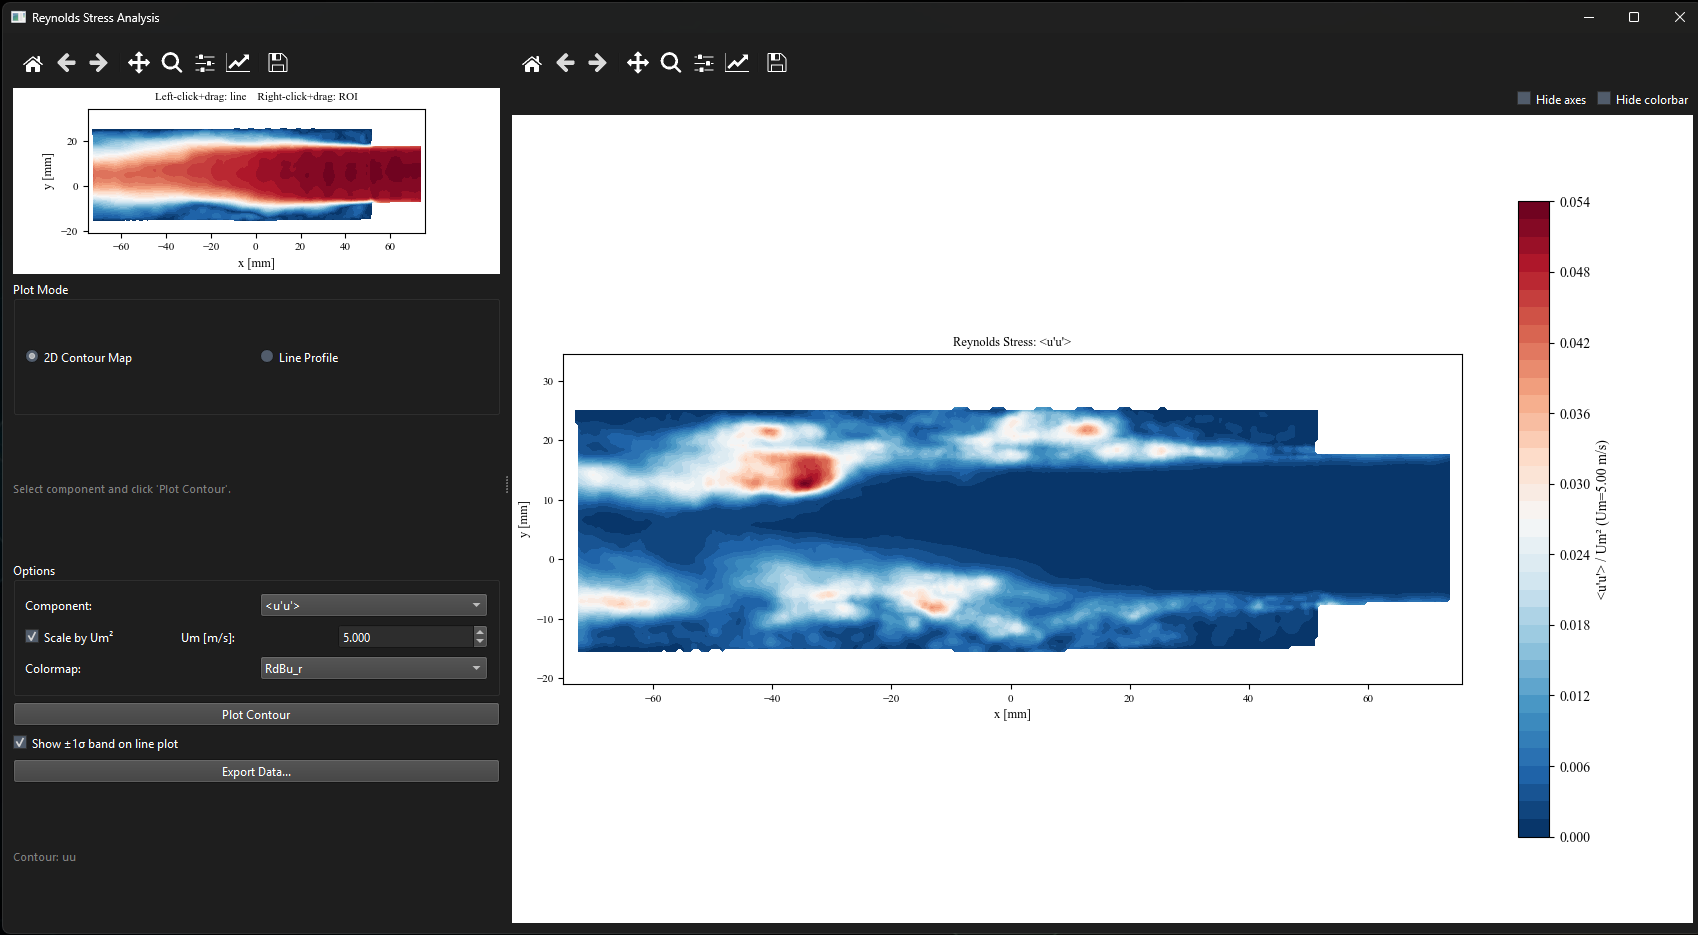
\includegraphics[width=0.92\linewidth]{fig2}
  \caption{Reynolds stress window in 2D contour mode showing $\langle u'v' \rangle$. The mean field is shown in the small reference panel on the left.}
  \label{fig:reynolds_contour}
\end{figure}

\subsection{Line profile}

\begin{quote}
\textbf{Important}
\begin{enumerate}[leftmargin=1.5em, topsep=2pt]
  \item Select `Line Profile` under Plot Mode.
  \item Choose line orientation: `Free`, `Horizontal`, or `Vertical`.
  \item For Horizontal/Vertical, set `Spatial avg $\pm$ pts` to average over neighboring rows or columns and reduce noise.
  \item Left-click and drag on the left field panel to draw the line, \emph{or} type the endpoint coordinates $(x_0, y_0)$ and $(x_1, y_1)$ into the `Line coordinates` boxes and click `Set Line` to place the line exactly (v0.7.0). Manual entry is useful for reproducing the same line across cases or datasets.
  \item Click `Plot Line Profile`.
\end{enumerate}
\end{quote}

All available stress components are plotted together. Check `Show $\pm1\sigma$ band` to display uncertainty bands. From v0.5.0 onward this checkbox is unchecked by default; the bands tend to crowd plots when multiple cases are overlaid for comparison.

\begin{figure}[htbp]
  \centering
  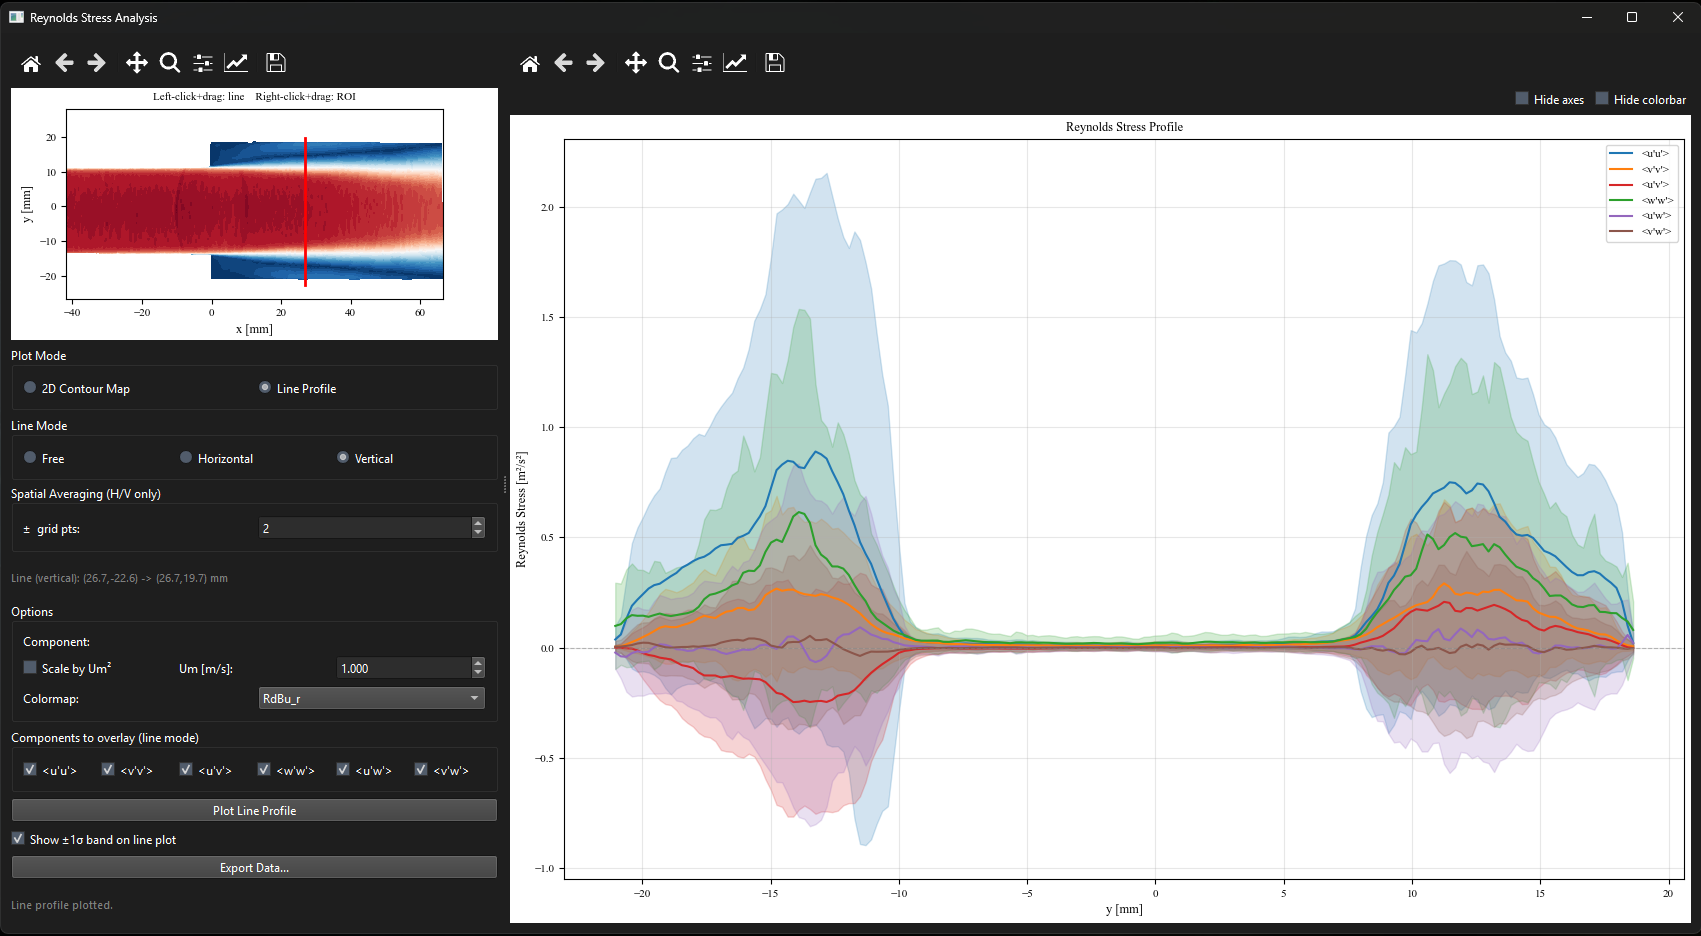
\includegraphics[width=0.92\linewidth]{fig3}
  \caption{Reynolds stress window in line profile mode. All stress components are plotted simultaneously in different colors. Optional shaded bands show $\pm 1\sigma$ statistical uncertainty (toggle in the side panel).}
  \label{fig:reynolds_profile}
\end{figure}

\begin{figure}[htbp]
  \centering
  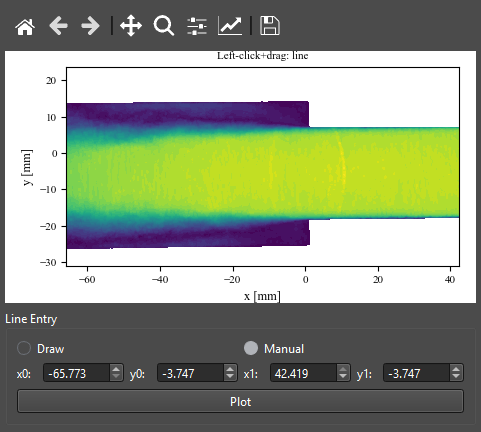
\includegraphics[width=0.6\linewidth]{fig_coord_entry}
  \caption{Manual line-coordinate entry (v0.7.0). In any Line Profile mode the endpoints can be set numerically as $(x_0, y_0)$ and $(x_1, y_1)$ instead of, or in addition to, click-and-drag. The same coordinate boxes appear in Reynolds Stress, TKE Budget, and Mean Velocity line profiles, so an identical line can be reproduced exactly across datasets.}
  \label{fig:coordentry}
\end{figure}

\subsection{Multi-case comparison}

The Reynolds Stress window supports importing CSV exports from previous sessions and overlaying them on the current plot. See Chapter~\ref{ch:multicase} for the full workflow. The same Import Case, Edit Styles, Manage Cases, and Export All Cases controls apply.

\subsection{Exporting}

Click `Export Data\ldots` to save all stress components simultaneously in a single Tecplot \texttt{.dat} file or as a CSV.

% ============================= CHAPTER 6 ==============================
